% concatenated from main.tex
\documentclass[onecolumn]{IEEEtran}
% -----------------------------------------------------------------------------
% Packages
% -----------------------------------------------------------------------------
\usepackage{amsmath,amssymb,amsthm,mathtools}
\mathtoolsset{showonlyrefs}
\usepackage{cite}
\usepackage{graphicx}
\usepackage[hidelinks]{hyperref}
\usepackage{tikz}
\usetikzlibrary{arrows.meta,decorations.pathmorphing}
\usepackage{enumerate}
%\usepackage{refcheck}

\usepackage{setspace}
\usepackage{verbatim}
%\doublespacing

% Commands and theorem environments
% -----------------------------------------------------------------------------
\newcommand{\R}{\mathbb{R}}
\newcommand{\GOE}{\operatorname{GOE}}

\newcommand{\avg}[1]{\left\langle #1\right\rangle}

\newcommand{\dd}{\mathop{}\!\mathrm{d}}

\newtheorem{theorem}{Theorem}
\newtheorem{lemma}[theorem]{Lemma}
\newtheorem{proposition}[theorem]{Proposition}
\newtheorem{corollary}[theorem]{Corollary}
\newtheorem{remark}[theorem]{Remark}

% -----------------------------------------------------------------------------
% Title and authors
% -----------------------------------------------------------------------------
\title{Gain of Entrainment in Nonlinear Cascades }

\author{Ram~Massas and Michael~Margaliot%
\thanks{RM and MM are with the School of Electrical Engineering,
Tel Aviv University, Tel Aviv 69978, Israel.
Corresponding author: Michael Margaliot (michaelm@tauex.tau.ac.il).}%
\thanks{The research of MM  was partially supported by the Israel Science
Foundation under Grant 221/24.}}
\usepackage{amsthm}
\newtheorem{example}[theorem]{Example}

\begin{document}

\maketitle



\begin{abstract}
%%%%%%%
We consider the gain of entrainment (GOE)--the difference between the average steady-state output under a periodic input and the steady-state output under a constant input with the same mean--for an $n$-stage feedforward cascade of stable first-order filters interleaved with static nonlinearities. The main result is an exact decomposition of~GOE as a weighted sum of local Jensen gaps, where each gap quantifies the mean shift generated by a  nonlinearity, and each weight is a product of downstream incremental  gains divided by linear time constants. We provide a Bregman-divergence interpretation of the decomposition, and a  second-order small-amplitude of GOE separating local curvature, fluctuation energy, and differential gains.
We demonstrate the theoretical results using a Michaelis–Menten cascade showing that any nonconstant periodic feeding strictly reduces the average terminal product relative to constant feeding with the same mean.
\end{abstract}

\begin{IEEEkeywords}
Bregman divergence, convexity, entrainment, Jensen gap,
 periodic forcing, chemical reaction network.
\end{IEEEkeywords}

% =============================================================================
% =============================================================================
% =============================================================================
\section{Introduction}
\label{sec:introduction}
% =============================================================================

Many natural and artificial systems and processes are subject to $T$-periodic excitation or forcing, and 
their proper functioning requires synchronization or entrainment to a $T$-periodic  behavior pattern. Synchronous generators must entrain to the frequency of the grid. Internal clocks in biological organisms must entrain to the 24-hour solar day.  
Phase-locked loops synchronize to periodic reference signals, and
cardiac pacemaker cells synchronize to periodic electrical stimulation. 



Entrainment is by no means a generic property of nonlinear systems~\cite{NIKOLAEV20181232,takac_sub_harmonics}.
However, there are important classes   of dynamical systems that do  entrain to periodic excitations. These include contractive systems~\cite{AminzareSontag2014,Russo2010}, totally positive differential systems~\cite{TPDS_MAR_SONATG},
and monotone dynamical systems with a first integral~\cite{Ji-Fa-periodic}. 
 

Entrainment raises the question of whether periodic forcing can do more than
induce synchronization, namely, whether it can also enhance system performance.
%%
The concept of \emph{gain of entrainment}~(GOE) allows  addressing  this question in a rigorous manner. To explain this, consider the nonlinear dynamical system 
\begin{align} \label{eq:nonlinsys}
\dot x&=f(x,u), \nonumber \\
y&=h(x,u),
\end{align}
with state
vector \(x\), input \(u\), and a scalar performance output~$y$.
The system is said to \emph{entrain} if for any \(T\)-periodic input \(u\)  any solution of~\eqref{eq:nonlinsys} converges to a unique~$T$-periodic limit cycle~$\gamma^u$, and thus the output converges to  the $T$-periodic output
\[
y^\gamma(t):=h(\gamma^u(t),u(t)).
\]
Suppose that the objective is to maximize the output. Since this converges to~$y^\gamma$, it is natural to consider the time average
\[
\avg{y^\gamma} := \frac{1}{T}\int_0^T h(\gamma^u(t),u(t))\,dt.
\]
As an illustration, the output may represent the average traffic flow through a
road network regulated by periodically varying traffic lights, and the goal is   
to maximize throughput. As another example, the output may represent the product yield of a chemical reactor operated under   periodic     feeding.


Let
\[
\avg{u}:=\frac1T\int_0^T u(t)\,dt
\]
denote the mean value of the input.
Since the system entrains, when  the constant input \(\avg{u}\) is applied to~\eqref{eq:nonlinsys}, the state converges to an
equilibrium,  denoted~\(e^{\avg{u}}\), and  thus the output converges to  the constant value
\[
h(e^{\avg{u}},\avg{u}).
\]
The gain of entrainment associated with the $T$-periodic input \(u\) is then defined
by
\[
\GOE(u):=
\frac1T\int_0^T h(\gamma(t),u(t))\,dt
-h(e^{\avg{u}},\avg{u}).
\]
Hence, \(\GOE(v)>0\) means that redistributing the input periodically in time
improves the average output. Conversely,
\(\GOE(v)<0\) means that the temporal variation is detrimental relative to
constant operation, so in this  case entrainment allows 
synchronization to periodic signals, but at the cost of decreasing  the output, on average.


For stable linear dynamics with a linear output, the average periodic state
coincides with the equilibrium associated with the average input. Therefore,
the corresponding~GOE is zero. In nonlinear systems, the situation is more interesting. 
To demonstrate this, we consider
an example from Ref.~\cite{Pavlov2007}, that  studied the frequency response of convergent systems (that are closely related to contractive systems~\cite{RUFFER2013277}).  
\begin{example}\label{exa:nonlin_with_goe}
    Consider the non-linear system:    \begin{align}\label{eq:nolonpav}
    \dot x_1&=-x_1+x_2^2,\nonumber\\
    \dot x_2&=-x_2+u,\nonumber\\
    y&=x_1.
    \end{align}
This is the series interconnection of two (scalar)  contractive  systems,  and is thus a  contractive system (see, e.g.,~\cite{ofir2021sufficient}).
We compare the effect of two controls:
\begin{enumerate}
    \item  $u_1(t)=a\sin(\omega t)$, 
where~$  a,\omega>0$; and
\item 
$u_2(t)=0$.
 \end{enumerate}
%%%%
Note that $u_1$ is~$T$-periodic with~$T:=2\pi/\omega$,
and that~$u_2(t)=\avg{u_1}$.
%%
For the zero control  the state vector converges  to $e^{\avg{u_1}}=0$, so~$y(t)$ converges to zero. 
For the control~$u(t)=u_1(t) $,   a calculation shows that the state vector 
 converges to a $T$-periodic solution~$\gamma^{u_1}$ satisfying 
%%%%%%%%%%
\begin{equation*} 
s(\omega)
\gamma_1^{u_1}(t)= 4a^2\omega^2+a^2-2a^2\omega\sin(2t\omega-p(\omega))-a^2\cos( 2t\omega-p(\omega)),  
\end{equation*}
with~$s(\omega):=2(4\omega^4+5\omega^2+1) $ and~$p(\omega):=2\,
 \arctan (\omega)$,
%\tan^{-1}
so 
%%%%%%
$\frac{1}{T}\int_0^T \gamma_1^{u_1}
(t) \mathrm{d} t 
 = \frac{a^2 }{2(1+\omega^2)} 
$. Thus, 
\begin{align}\label{eq:GOE_ISQUAD}
\GOE(u_1)=\frac{a^2 }{2(1+\omega^2)} ,
\end{align}
which is  positive and depends on both  the excitation amplitude~$a$, and excitation
frequency~$\omega$. 

Note that $\GOE(u_1)$
decreases to zero as $\omega\to\infty$, reflecting the attenuation of high-frequency inputs by the stable
linear filter preceding the quadratic stage.
For a fixed $\omega$, the quadratic dependence of $\GOE(u_1)$ on the control amplitude~$a$ implies the following. If $a\ll 1$ [$a\gg 1$] then $\GOE(u_1)\ll a$ [$\GOE(u_1)\gg a$]. 
%%%%%%%%    
\end{example}


Since constant inputs form a special case of periodic inputs, one might expect
that~GOE is always nonnegative, yet this intuition is generally
incorrect. 
Analyzing~GOE is a challenging theoretical
problem 
because in general  nonlinear systems both~$\gamma^u$ and~$e^{\avg{u}}$ are not known explicitly. Maximizing~GOE can   be posed as  an optimal control problem with a constraint on the average control, but 
explicit solutions are known only in relatively simple settings, such as scalar
systems~\cite{rapo_convex}.
%%
%%

  GOE is important in 
  numerous applications 
 including periodically harvested fisheries, photobioreactors operated  by
time-varying light, traffic networks controlled by periodic signal timing,  
drug delivery protocols based on periodic  dosing schedules, gene expression  under periodic  regulation, and
manufacturing systems operating under cyclic production schedules.



In models of
protein translation, one may ask whether periodic variation of initiation or
elongation resources may increase the average production rate.  
Ref.~\cite{GOE_RFM_2023}  considered GOE
in an important nonlinear model from  systems biology called the ribosome flow model~(RFM). 
In this case, the scalar output corresponds to  the protein production rate in mRNA translation,
the $n$-dimensional  state vector corresponds to the densities of ribosomes along~$n$ different sections of the mRNA molecule, and 
and the~$(n+1)$-dimensional  input to the transition rates of ribosomes along different segments  of the mRNA molecule. The RFM is an (almost) contractive system~\cite{weak_contract}, and thus entrains to periodic  inputs~\cite{Margaliot2014Entrain}. 
It was shown in~\cite{GOE_RFM_2023} 
that in several special cases~$\GOE(u)\leq 0$. More recently, and using a different technique, Ref.~\cite{cost_of_entrain} proved that in the RFM we always  have~$\GOE(u)\leq 0$, with equality only in  the degenerate case 
where all the $T$-periodic transition rates are equal, up to multiplication by a positive constant.
Thus,~$\GOE(u)<0$
for any non-trivial periodic modulation, implying  that entrainment to periodic controls always comes with a cost in terms of the protein production rate. 

Ref.~\cite{Katz2024} 
  considered a class of 
  weakly contractive systems under a control~$u(t)=a+\varepsilon \tilde u(t)$, with~$\tilde u$ a $T$-periodic control and~$\varepsilon\in \R$.
  Using   a first-order expression
for the GOE, it was shown   that GOE is
inherently a second- or higher-order effect in~$\varepsilon$.
%%%
Ref.~\cite{MassasMargaliot_linear_sys_nonlin_output} investigated systems with
linear dynamics and a static nonlinear output map~$h$, establishing a connection between the
sign of~GOE and the convexity or concavity of~$h$.

Here, we consider   a   cascade (or serial connection) of scalar linear systems with a nonlinear output. Feedforward cascades are a common interconnection structure in engineering, biology, chemistry, communication systems,  and economics.
Understanding how local nonlinearities combine to determine global performance remains a fundamental challenge. 
We analyze GOE of such a cascade. 
This system is contractive, and thus entrains to periodic excitations.   
In a cascade with several nonlinear
stages, the situation is fundamentally different from that of  a single linear system with a nonlinear output~\cite{MassasMargaliot_linear_sys_nonlin_output},
as every nonlinear
stage may create its own mean displacement, and each displacement must then
propagate through all downstream stages before reaching the output.
A downstream stage may amplify or attenuate this displacement and may even reverse its sign. Consequently, the sign and magnitude
of the overall GOE cannot generally be determined by examining the curvature
of a single function.

 The main contributions of this paper are as follows. We derive an exact decomposition of  GOE in the cascade as  a sum of local contributions associated with each nonlinear stage and propagation weights determined by the downstream dynamics. This decomposition separates the generation of average shifts due to nonlinearity from their propagation through the cascade, providing a transparent stage-by-stage interpretation of GOE. We further establish sufficient conditions that determine the sign of the GOE, derive an equivalent representation based on Bregman divergences, and develop a second-order approximation that relates the GOE to the local curvature of the nonlinearities and the differential gains of the cascade. We illustrate the theoretical results  using  a cascade with Michaelis--Menten kinetics, demonstrating how the proposed framework explains the effect of periodic forcing on the average output.
 
%We use standard notation. 
For a $T$-periodic  function $q$,   let 
\[ 
    \avg q
    :=
    \frac{1}{T}\int_0^T q(t)\,\mathrm{d}t.
\]
Note that if~$q$  is $C^1$ then
 \begin{align}
     \label{eq:avgderiszero}
 \avg{\dot q}=\frac{1}{T}\int_0^T \dot q(t) \mathrm{d}t =\frac1{T}(q(T)-q(0) )=0. 
\end{align}

 
%%%%%%%%%%%%%%%%%
\section{Main Results}\label{sec:main}
%%%%%%%%%%%%%%%5
Consider the   $n$-stage feedforward cascade
\begin{align} \label{eq:cascade-general}
    \dot x_1(t)
    &=
    -a_1x_1(t)+\phi_1\bigl(u(t)\bigr),
    \nonumber\\
    \dot x_i(t)
    &=
    -a_ix_i(t)+\phi_i\bigl(x_{i-1}(t)\bigr),
    \qquad i=2,\ldots,n,
    \\
    y(t)
    &=
    x_n(t),\nonumber 
\end{align}
where~$a_i>0$  for all~$i$, and every~$\phi_i:\R\to\R$ is a continuous   function (and thus maps compact  sets to compact  sets). 
Each state is thus  a stable first-order dynamical filter driven by a
static nonlinear map of the signal arriving from the preceding
stage.

\begin{comment}
%%
The direction of signal propagation is
\begin{equation}
    v
    \longrightarrow
    \phi_1
    \longrightarrow
    x_1
    \longrightarrow
    \phi_2
    \longrightarrow
    x_2
    \longrightarrow
    \cdots
    \longrightarrow
    \phi_n
    \longrightarrow
    x_n=y.
    \label{eq:intro-signal-propagation}
\end{equation}
%%%
\end{comment}


Consider a continuous $T$-periodic   control~$v$. Then~$v$ takes values in a compact set, and thus so does~$\phi_1(v)$. This implies that~$x_1 $ is bounded and converges to a unique~$T$-periodic limit cycle~$\gamma_1^v$. Using this implies that~$x_2 $ is bounded and converges to a
unique~$T$-periodic limit cycle~$\gamma_2^v$. Continuing in this fashion, we have that for any initial condition~$x(0)$ the state~$x$ converges to a 
unique~$T$-periodic limit cycle~$\gamma^v$.

 
For the constant 
control~$u=\avg{v}$, the state 
$x$ converges to an  equilibrium $e^{\avg{v}}$ with 
\begin{align*}
e_1^{\avg{ v}}& = a_1 ^{-1} \phi_1(  \avg {v}),\nonumber\\
e_i^{\avg{ v} }&= a_i ^{-1} \phi_i (
 e_{i-1}^{\avg{v}}) ,
\quad   i=2,\dots,n.
\end{align*}

Since the output is $y=x_n$, we get that   
\begin{equation}
    \GOE(v)
    =
    \frac{1}{T}
    \int_{0}^{T}\gamma_n^v(t)\,\mathrm{d}t
    -
    e_n^{\avg{ v}}
    =
    \avg{\gamma_n^v}
    -
    e_n^{\avg{ v}}.
    \label{eq:intro-cascade-goe}
\end{equation}

 Note that for the cascade \eqref{eq:cascade-general} 
 it is possible in general to give an explicit \emph{integral representation} for each $\gamma_i^v$, but not   a closed-form elementary expression.

 \begin{comment}
      \begin{example}    
A hydraulic analogy of the cascade is presented in
Fig.~\ref{fig:cascade-schematic}. Each tank represents a dynamical state
\(x_i\), whereas each funnel labeled \(\phi_i\) represents the nonlinear
transformation applied before the signal enters the corresponding state.
The dashed lateral arrows represent the linear dissipation terms \(a_ix_i\).
The vertical arrangement emphasizes the feedforward propagation of the
periodic signal from \(v(t)\) to the measured output \(y(t)=x_n(t)\).
\end{example}

% End the current page before displaying the figure.
\clearpage

\begin{figure}[!t]
\centering

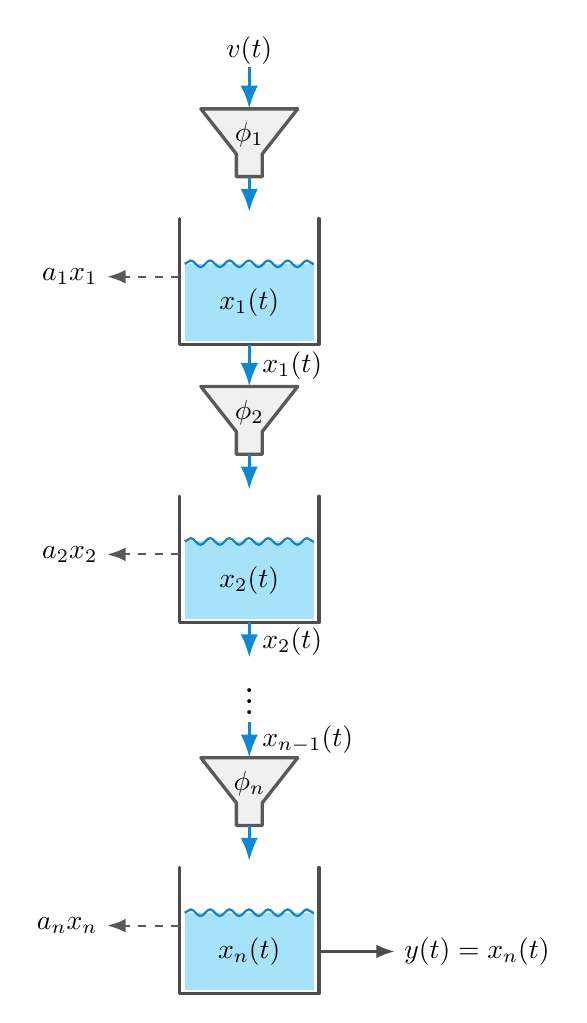
\begin{tikzpicture}[
    scale=0.82,
    >=Latex,
    flow/.style={
        ->,
        very thick,
        draw=cyan!70!blue
    },
    loss/.style={
        ->,
        dashed,
        thick,
        draw=black!65
    },
    output/.style={
        ->,
        thick,
        draw=black!70
    },
    tank/.style={
        very thick,
        draw=black!70,
        line cap=round,
        line join=round
    },
    water/.style={
        fill=cyan!35,
        draw=none
    },
    surface/.style={
        cyan!65!blue,
        thick,
        decorate,
        decoration={
            snake,
            amplitude=1.2pt,
            segment length=7pt
        }
    },
    every node/.style={
        font=\normalsize
    }
]

% ==========================================================
% Input and first nonlinear map
% ==========================================================

\node at (0,0.25) {$v(t)$};

\draw[flow] (0,0) -- (0,-0.65);

% Funnel phi_1
\filldraw[
    fill=gray!12,
    draw=black!65,
    very thick,
    line join=round
]
(-0.75,-0.65)
--
(0.75,-0.65)
--
(0.20,-1.35)
--
(0.20,-1.70)
--
(-0.20,-1.70)
--
(-0.20,-1.35)
--
cycle;

\node at (0,-1.05) {$\phi_1$};

\draw[flow] (0,-1.70) -- (0,-2.25);

% ==========================================================
% First tank
% ==========================================================

\fill[water]
(-1.00,-3.05)
rectangle
(1.00,-4.25);

\draw[surface]
(-1.00,-3.05)
--
(1.00,-3.05);

\draw[tank]
(-1.08,-2.35)
--
(-1.08,-4.30)
--
(1.08,-4.30)
--
(1.08,-2.35);

\node at (0,-3.65) {$x_1(t)$};

% Dissipation from first tank
\draw[loss]
(-1.08,-3.25)
--
(-2.20,-3.25);

\node[left] at (-2.20,-3.25) {$a_1x_1$};

% Flow from x_1 to phi_2
\draw[flow]
(0,-4.30)
--
(0,-4.95);

\node[right] at (0.05,-4.62) {$x_1(t)$};

% ==========================================================
% Second nonlinear map
% ==========================================================

\filldraw[
    fill=gray!12,
    draw=black!65,
    very thick,
    line join=round
]
(-0.75,-4.95)
--
(0.75,-4.95)
--
(0.20,-5.65)
--
(0.20,-6.00)
--
(-0.20,-6.00)
--
(-0.20,-5.65)
--
cycle;

\node at (0,-5.35) {$\phi_2$};

\draw[flow]
(0,-6.00)
--
(0,-6.55);

% ==========================================================
% Second tank
% ==========================================================

\fill[water]
(-1.00,-7.35)
rectangle
(1.00,-8.55);

\draw[surface]
(-1.00,-7.35)
--
(1.00,-7.35);

\draw[tank]
(-1.08,-6.65)
--
(-1.08,-8.60)
--
(1.08,-8.60)
--
(1.08,-6.65);

\node at (0,-7.95) {$x_2(t)$};

% Dissipation from second tank
\draw[loss]
(-1.08,-7.55)
--
(-2.20,-7.55);

\node[left] at (-2.20,-7.55) {$a_2x_2$};

% Flow toward the remaining stages
\draw[flow]
(0,-8.60)
--
(0,-9.15);

\node[right] at (0.05,-8.90) {$x_2(t)$};

% Remaining intermediate stages
\node at (0,-9.70) {\Large $\vdots$};

\draw[flow]
(0,-10.15)
--
(0,-10.70);

\node[right] at (0.05,-10.42) {$x_{n-1}(t)$};

% ==========================================================
% Final nonlinear map
% ==========================================================

\filldraw[
    fill=gray!12,
    draw=black!65,
    very thick,
    line join=round
]
(-0.75,-10.70)
--
(0.75,-10.70)
--
(0.20,-11.40)
--
(0.20,-11.75)
--
(-0.20,-11.75)
--
(-0.20,-11.40)
--
cycle;

\node at (0,-11.10) {$\phi_n$};

\draw[flow]
(0,-11.75)
--
(0,-12.30);

% ==========================================================
% Final tank
% ==========================================================

\fill[water]
(-1.00,-13.10)
rectangle
(1.00,-14.30);

\draw[surface]
(-1.00,-13.10)
--
(1.00,-13.10);

\draw[tank]
(-1.08,-12.40)
--
(-1.08,-14.35)
--
(1.08,-14.35)
--
(1.08,-12.40);

\node at (0,-13.70) {$x_n(t)$};

% Dissipation from final tank
\draw[loss]
(-1.08,-13.30)
--
(-2.20,-13.30);

\node[left] at (-2.20,-13.30) {$a_nx_n$};

% Output
\draw[output]
(1.08,-13.70)
--
(2.25,-13.70);

\node[right] at (2.25,-13.70) {$y(t)=x_n(t)$};

\end{tikzpicture}

\caption{Hydraulic analogy of the nonlinear cascade
\eqref{eq:cascade-general}.
Each tank represents a dynamical state \(x_i\), each funnel represents the
nonlinear map \(\phi_i\), and the dashed lateral arrows represent the
dissipative terms \(a_ix_i\). The illustration describes the direction of
signal propagation and is not intended to represent a physical
mass-conservation model.}
\label{fig:cascade-schematic}

\end{figure}

% Ensure that the figure is printed before the text continues.
\clearpage

The hydraulic analogy also illustrates the two operations performed at every
stage. The incoming signal is first transformed by the static nonlinear map
\(\phi_i\), and the transformed signal then drives a stable first-order
filter. Although the dynamical equation of each individual state is linear
in that state, the cascade as a whole is nonlinear because the forcing of
each stage depends nonlinearly on the preceding signal.

 \end{comment}

\begin{comment}
    
The first nonlinearity \(\phi_1\) is an essential part of the model. Defining
a new signal \(u(t):=\phi_1(v(t))\) would generally change the mean-constrained
comparison because
\begin{equation}
    \avg{\phi_1(v)}
    \neq
    \phi_1\bigl(\avg{v}\bigr).
\end{equation}
Thus, absorbing \(\phi_1\) into a redefined input would remove precisely one
of the nonlinear averaging effects that contributes to the GOE.

 % =============================================================================
\section{Problem Formulation}
% =============================================================================

Let $v:\R_{\geq0}\to\R$ be a continuous, $T$-periodic input, and let
\begin{equation*}
    \bar v
    :=
    \avg{v}
    :=
    \frac{1}{T}\int_0^T v(t)\,\mathrm{d}t.
    \label{eq:input-average}
\end{equation*}
Assume throughout that
\begin{equation}
    a_i>0,
    \qquad
    \phi_i:\R\to\R\text{ is continuous},
    \qquad i=1,\ldots,n.
    \label{eq:basic-assumptions}
\end{equation}

The mean constraint is imposed on the externally prescribed signal $v$
itself. Although one may define an effective actuation
$u(t):=\phi_1(v(t))$, this transformation does not generally preserve the
GOE comparison, since
\begin{equation}
    \avg{\phi_1(v)}
    \neq
    \phi_1(\avg{v})
\end{equation}
in general. Thus, the input nonlinearity $\phi_1$ cannot be absorbed into a
redefined control without changing the mean-constrained problem.
 
We show below that the periodic input $v$ induces a unique globally attracting
$T$-periodic solution
\begin{equation}
    \gamma^v(t)
    =
    \bigl(
    \gamma_1^v(t),\ldots,\gamma_n^v(t)
    \bigr)^\top.
\end{equation}
The GOE associated with $v$ is therefore well defined by
\begin{equation}
    \GOE(v)
    :=
    \frac{1}{T}
    \int_0^T\gamma_n^v(t)\,\mathrm{d}t
    -
    e_n^{\bar v}.
    \label{eq:goe-definition}
\end{equation}
The comparison is fair in the sense that $v$ and the constant input $\bar v$
have the same time average.

% =============================================================================
\section{Entrainment of the Cascade}
% =============================================================================

We first establish the existence, uniqueness, and global attractivity of the
periodic response used in \eqref{eq:goe-definition}.

\begin{lemma}
\label{lem:scalar-filter}
Consider
\begin{equation}
    \dot z(t)=-az(t)+p(t),
    \qquad a>0,
    \label{eq:scalar-filter}
\end{equation}
where $p$ is continuous and $T$-periodic. Then
\eqref{eq:scalar-filter} admits a unique $T$-periodic solution $\gamma^p$,
and every solution satisfies
\begin{equation}
    |z(t)-\gamma^p(t)|
    =
    e^{-at}|z(0)-\gamma^p(0)|.
    \label{eq:filter-contraction}
\end{equation}
\end{lemma}

\begin{proof}
Variation of constants gives
\begin{equation}
    z(t)
    =
    e^{-at}z(0)
    +
    \int_0^t e^{-a(t-s)}p(s)\,\mathrm{d}s.
\end{equation}
The condition $z(T)=z(0)$ determines exactly one initial value,
\begin{equation}
    z_\star
    =
    \frac{
    \displaystyle
    \int_0^T e^{-a(T-s)}p(s)\,\mathrm{d}s
    }{
    1-e^{-aT}
    }.
    \label{eq:periodic-initial}
\end{equation}
The solution initialized at $z_\star$ is $T$-periodic by periodicity of $p$
and uniqueness of solutions. The difference of any two solutions satisfies
$\dot r=-ar$, yielding \eqref{eq:filter-contraction}. This proves uniqueness
and global attractivity.
\end{proof}

\begin{theorem}
\label{thm:entrainment}
Under \eqref{eq:basic-assumptions}, every continuous $T$-periodic input $v$
induces a unique $T$-periodic solution $\gamma^v$ of
\eqref{eq:cascade-first}--\eqref{eq:cascade-general}. Moreover,
\begin{equation}
    \lim_{t\to\infty}
    \left\|x(t)-\gamma^v(t)\right\|
    =
    0
    \label{eq:global-attraction}
\end{equation}
for every initial condition.
\end{theorem}

\begin{proof}
Since $\phi_1(v(t))$ is continuous and $T$-periodic,
Lemma~\ref{lem:scalar-filter} yields a unique periodic solution
$\gamma_1^v$ for the first stage. Suppose that $\gamma_{i-1}^v$ has already
been constructed. Then
\begin{equation}
    p_i(t)
    :=
    \phi_i(\gamma_{i-1}^v(t))
\end{equation}
is continuous and $T$-periodic. Applying Lemma~\ref{lem:scalar-filter}
recursively for $i=2,\ldots,n$ constructs a $T$-periodic solution of the
entire cascade. The same forward induction and uniqueness in
Lemma~\ref{lem:scalar-filter} show that no second periodic solution can exist.

It remains to prove global attraction. Let
\begin{equation}
    r_i(t):=x_i(t)-\gamma_i^v(t).
\end{equation}
For the first stage,
\begin{equation}
    r_1(t)=e^{-a_1t}r_1(0)\to0.
\end{equation}
Suppose that $r_{i-1}(t)\to0$. Then
\begin{equation}
    \dot r_i=-a_ir_i+q_i(t),
    \label{eq:error-recursion}
\end{equation}
where
\begin{equation}
    q_i(t)
    :=
    \phi_i(x_{i-1}(t))
    -
    \phi_i(\gamma_{i-1}^v(t)).
\end{equation}
The induction hypothesis implies that $x_{i-1}$ is eventually contained in
a compact neighborhood of the bounded periodic signal $\gamma_{i-1}^v$.
Uniform continuity of $\phi_i$ on this compact set yields $q_i(t)\to0$.
Variation of constants gives
\begin{equation}
    r_i(t)
    =
    e^{-a_it}r_i(0)
    +
    \int_0^t e^{-a_i(t-s)}q_i(s)\,\mathrm{d}s.
\end{equation}
The convolution of a stable exponential kernel with a bounded signal tending
to zero also tends to zero. Hence $r_i(t)\to0$. Forward induction proves
\eqref{eq:global-attraction}.
\end{proof}
\end{comment}

 
% =============================================================================
\subsection{Formula for GOE}
% 
Define the mean displacement at stage $i$ by
\begin{equation}
    \Delta_i(v)
    :=
    \avg{\gamma_i^v}-e_i^{\avg{ v}},
    \qquad i=1,\ldots,n.
    \label{eq:delta-def}
\end{equation}
By \eqref{eq:intro-cascade-goe},
\begin{equation}
    \GOE(v)=\Delta_n(v).
    \label{eq:goe-delta}
\end{equation}

It is useful to define
\begin{equation}\label{eq:gamm0}
\gamma_0^v(t) := v(t).
\end{equation}
To identify the     contributions of the nonlinear functions, define
\begin{align}  \label{eq:jensen-internal}
    J_i(v)
    &:=
    \avg{\phi_i(\gamma_{i-1}^v)}
    -
    \phi_i\bigl(\avg{\gamma_{i-1}^v}\bigr),
    \qquad i=1,\ldots,n.
\end{align}
Thus, $J_i$ is the Jensen gap generated at stage $i$ by $\phi_i$.
%%
For every internal stage $i=2,\ldots,n$, define the incremental
gain $  L_i(v)$ by
%%%%%%%%%%%%
\begin{equation}\label{eq:secant-gain} 
    L_i(v)
    :=
    \dfrac{
    \phi_i(\avg{\gamma_{i-1}^v})
    -
    \phi_i(e_{i-1}^{\avg {v}})
    }{
    \Delta_{i-1}(v)
    },
\end{equation} 
if 
$ \Delta_{i-1}(v)\neq0$,
and~$L_i(v)=0$, otherwise.
This   ensures that
\begin{equation}\label{eq:ensuresthat}
    \phi_i(\avg{\gamma_{i-1}^v})
    -
    \phi_i(e_{i-1}^{\avg {v}})
    =
    L_i(v)\Delta_{i-1}(v)
\end{equation}
also when $\Delta_{i-1}(v)=0$.
If~\eqref{eq:secant-gain} is well-defined also when~$\Delta_{i-1}(v)=0$ then   the definition~\eqref{eq:secant-gain} is used for all~$v$. 
 Our first main result provides a formula for~$\GOE(v)$ 
as a weighted sum of~$J_k(v)$, $k=1,\dots,n$.
%%%%%%%
We can now state our first main result. 
\begin{theorem}[Formula for GOE of  a cascade]
\label{thm:exact-decomp}
For every continuous $T$-periodic input $v$, we have 
\begin{equation}  \label{eq:exact-goe}
     \GOE(v)
    =
    \sum_{k=1}^n W_k(v)J_k(v)
    ,
\end{equation}
where
\begin{equation}
    W_k(v)
    :=
    {a_k} ^{-1}
    \prod_{j=k+1}^n
 {a_j}  ^{-1} {L_j(v)} ,
    \qquad k=1,\ldots,n, 
    \label{eq:cascade-weight}
\end{equation}
with the convention that an empty product equals~$1$.
\end{theorem}

Eq.~\eqref{eq:exact-goe} separates two mechanisms determining~GOE. The \emph{local term}
$J_k$ measures the mean shift  created  by the curvature of $\phi_k$,
whereas the weight~$W_k$ measures how this shift is \emph{propagated} from stage~$k$
through the downstream stages~$k+1,\ldots,n$ to the output. In particular,
a negative downstream   gain reverses the sign of every contribution
that passes through it. 
 
\begin{proof}
Averaging the first equation of the cascade along the periodic orbit gives
$
    0
    =
    -a_1\avg{\gamma_1^v}
    +
    \avg{\phi_1(v)}.
$
Subtracting the identity 
$    0
    =
    -a_1e_1^{\avg {v}}
    +
    \phi_1(\avg {v})
$ yields
\begin{equation}
    \Delta_1(v)
    =a_1^{-1}
    {J_1(v)} .
    \label{eq:delta-first}
\end{equation}
%%%
For $i=2,\ldots,n$, periodic averaging and subtraction of the corresponding
equilibrium equation give
\begin{align*}
    a_i\Delta_i(v)
    &=
    \avg{\phi_i(\gamma_{i-1}^v)}
    -
    \phi_i(e_{i-1}^{\avg {v}})
    \nonumber\\
    &=
    J_i(v)
    +
    \phi_i(\avg{\gamma_{i-1}^v})
    -
    \phi_i(e_{i-1}^{\avg {v}})
    \nonumber\\
    &=
    J_i(v)+L_i(v)\Delta_{i-1}(v), 
\end{align*}
where the last step follows from \eqref{eq:ensuresthat}. Thus,  
\begin{equation*}
    \Delta_i(v)
    =a_i^{-1} \left (
    J_i(v)
    +
    L_i(v)\Delta_{i-1}(v) \right).
    \label{eq:delta-recursion2}
\end{equation*}
Starting from \eqref{eq:delta-first}, expanding the recursion forward to
$i=n$, and using \eqref{eq:goe-delta} yields \eqref{eq:exact-goe}.
\end{proof}

 


\begin{example}
    Consider   again system~\eqref{eq:nolonpav} in Example~\ref{exa:nonlin_with_goe}. 
Define
   $ \xi_1:=x_2$ and
    $\xi_2:=x_1$.
Then  
\begin{align}\label{eq:samae}
    \dot \xi_1(t)
    &=
    -\xi_1(t)+u(t),\nonumber\\
    \dot \xi_2(t)
    &=
    -\xi_2(t)+\xi_1^2(t),\nonumber\\
    y(t)&=\xi_2(t),
\end{align}
which is   of the form
\eqref{eq:cascade-general} with~$n=2$, 
$\phi_1(s)=s$, $\phi_2(s)=s^2$, and~$a_1=a_2=1$.
In this case,
\[
J_1(u)=  \avg{\phi_1(u)}-\phi_1(\avg{ u})=0,
\]
and~\eqref{eq:exact-goe} 
gives
\begin{align*}
    \GOE (u) &= W_1(u) J_1(u)+W_2(u) J_2(u) \\
          &=     J_2(u)\\
          &=
       \avg{\phi_2(\gamma_{1}^u)}
    -
    \phi_2\bigl(\avg{\gamma_{1}^u}\bigr)\\
    & =   \avg{ (\gamma_{1}^u)^2}
    -
 \avg{\gamma_{1}^u} ^2
    .
\end{align*}

Let
    $u_1(t)=a\sin(\omega t)$, with~$a,\omega>0$. This is  $T$-periodic with~$T:=2\pi/\omega$. 
 The corresponding 
 unique periodic solution of~\eqref{eq:samae} 
 satisfies
\begin{align*}
    \gamma_1^{u_1}(t)
    &=
    \frac{a}{1+\omega^2}\sin(\omega t)
    -
    \frac{a\omega}{1+\omega^2}\cos(\omega t).
    \label{eq:gamma2-positive}
\end{align*}
 %%%
This gives  $\avg{\gamma_1^{u_1}}=0$,   
and
  $  \avg{(\gamma_1^{u_1})^2}
    =    \frac{a^2}{2(1+\omega^2)}$,
    so
\begin{equation*} 
    \GOE(u_1)
    =
    \frac{a^2}{2(1+\omega^2)}
     ,
\end{equation*}
and this agrees with~\eqref{eq:GOE_ISQUAD}. 
%%%%%
\end{example}

\begin{remark}
    If for some index $k$ the function $\phi_k$   is affine then \eqref{eq:jensen-internal} implies that
$J_k(v) =0 $ and Thm. \ref{thm:exact-decomp} implies that the $k$th stage in the cascade    contributes  no local Jensen gap to GOE (but it may still transmit, amplify, attenuate, or reverse upstream contributions).
\end{remark}


An important consequence of Theorem~\ref{thm:exact-decomp} is that it yields simple sufficient conditions guaranteeing the sign of the GOE in a cascade. Notably, these conditions can be verified without computing the equilibrium nor the periodic limit cycle. The following example demonstrates this.

 
 
\begin{corollary}
\label{cor:sign}
Suppose that  the functions~$\phi_1,\ldots,\phi_n$ are convex [concave], and that the functions 
$\phi_2,\ldots,\phi_n$ are nondecreasing. Then
    $\GOE(v) \geq 0$
[$\GOE(v)\leq 0$] for every continuous periodic input~$v$. 
\end{corollary}

\begin{proof}
%%%%
We prove the result for the case where all the~$\phi_k$s are convex.   Jensen's inequality 
gives~$J_k(v)\geq0$ for every~$k$.
The assumption that $\phi_2,\ldots,\phi_n$ are nondecreasing gives   
  $L_j(v)\geq0$ for $j=2,\ldots,n$, so all the weights
$W_k(v)$ are nonnegative. Now~\eqref{eq:exact-goe}  gives~$\GOE(v)\geq0$.
%%
\end{proof}

In general, convexity [concavity]  properties of the~$\phi_k$s are not enough to deduce the sign of GOE, due to the effect of the~$L_j$s.  
\begin{example}[Convex $\phi_i$s yet negative GOE]
\label{exa:negative}
Consider the two-stage cascade
\begin{align*}
    \dot x_1
    &=
    -x_1+v^2,
   \\
    \dot x_2
    &=
    -x_2-x_1,\\
 y&=x_2, 
   %%%%%%
\end{align*}
which is   of the form
\eqref{eq:cascade-general} with~$n=2$, 
$\phi_1(s)=s^2$, $\phi_2(s)=-s$, and~$a_1=a_2=1$.
 Note that both $\phi_i$s
are convex. 
In this case, $\phi_2$ is affine, so~$J_2=0$
and~\eqref{eq:exact-goe} 
gives
\begin{align*}
    \GOE (u) &= W_1(u) J_1(u)+W_2(u) J_2(u) \\
          &=     L_2(u) J_1(u)\\
          &=-J_1(u).
\end{align*}


Consider the control
$
    v(t)=a\sin(\omega t),
 $ with~$    a,\omega>0$.  Then 
 $
    J_1(v)
    =
    \avg{v^2}
    =
    a^2/2$,
    so $
    \GOE(v)
    =
    - {a^2}/{2}
    <0$.
Thus, the positive Jensen gap created by the strictly convex upstream map~$\phi_1$ is sign-reversed by the decreasing downstream map~$\phi_2$.
\end{example}

The proof of 
Corollary~\ref{cor:sign} 
suggests simple conditions guaranteeing  strict positivity [negativity] of~GOE. The next remark demonstrates this.

\begin{remark}[Strict positivity of GOE]
\label{rem:strict}
Suppose that the functions~$\phi_1,\ldots,\phi_n$ are convex,   that the functions 
$\phi_2,\ldots,\phi_n$ are nondecreasing, 
and that there
 exists an index $k$ such that
   $ J_k(v)>0$, 
and
 $   L_j(v)>0$,
    for~$ j=k+1,\ldots,n$.
Then $\GOE(v)>0$. 
(Note that~$J_k(v)>0$ whenever~$\phi_k$ is strictly convex on the range of
its periodic argument,
and that argument is nonconstant.)
\end{remark}

 

% =============================================================================
\subsection{Bregman-Divergence Representation}
% =============================================================================
Recall that if~\(g:\mathbb R^n\to\mathbb R\) is $C^1$  
then the function~$D_g:\R^n\times\R^n\to\R$
defined by
\begin{equation}\label{eq:d_geq}
D_g(x,z):=
g(x)-g(z)-(\nabla g(z))^\top (x-z) 
\end{equation}
is called the
Bregman divergence associated with~\(g\)~\cite{bregman1967}.
Geometrically, $D_g(x,z)$
  measures how much the graph of $g$ lies above its tangent plane at~$z$. 
The function~$D_g$
     is generally
neither symmetric nor a metric, but its sign is directly related to the
curvature of the underlying function. In particular, it is nonnegative for
convex functions,  and nonpositive for concave functions~\cite{bregman1967}.


Suppose now that~$\phi:\R\to\R$ is~$C^1$, and 
let $u$ be a scalar $T$-periodic control.
Fix $t\in[0,T)$. Then
\begin{align*}
%%%%
D_\phi(u(t),\avg{u})&=
\phi(u(t))-\phi(\avg{u})
-\phi'(\avg {u})(u(t)-\avg{u}),
\end{align*}
so
\begin{align*}
%%%%
\avg{D_\phi(u(t),\avg{u}) }&=
\avg {\phi(u)}-\phi(\avg{u}).
\end{align*}
Comparing this with \eqref{eq:jensen-internal} and using Theorem~\ref{thm:exact-decomp} yields the following result.

\begin{corollary}
[Geometric decomposition for GOE.]
\label{prop:bregman} 
Suppose  that all the~$\phi_i$s are~$C^1$, and
define the local average Bregman terms by
\begin{align}\label{eq:big_b}
    B_i(v)
    &:=
    \avg{
    D_{\phi_i}
    \bigl(
    \gamma_{i-1}^v,
    \avg{\gamma_{i-1}^v}
    \bigr)
    },
    \qquad i=1,\ldots,n.
 \end{align}
Then
\begin{equation}
    \GOE(v)
    =
    \sum_{k=1}^n W_k(v)B_k(v).
    \label{eq:bregman-goe}
\end{equation}
\end{corollary}

          
Thus,  every stage creates a local geometric discrepancy, and the
downstream part of the cascade propagates  this discrepancy to the output
through the weight $W_k$.

% =============================================================================
\subsection{Small-Amplitude Periodic Excitations}
\label{sec:small-amplitude}
% =============================================================================

We next study the local behavior of GOE in \eqref{eq:cascade-general} under small periodic
perturbations of a constant control.   
Consider the control 
\begin{equation}
    v_\varepsilon(t)
    =
    a +\varepsilon w(t),
    \label{eq:small-input}
\end{equation}
where $w$ is continuous and     $T$-periodic with $ \avg{w}=0$, and $\varepsilon\in\R$. Thus,~$\avg{v_\varepsilon}=a$. 
To simplify the notation, let 
\begin{equation*}
    \gamma^\varepsilon(t)
    :=
    \gamma^{v_\varepsilon}(t)
\end{equation*}
denote the unique $T$-periodic solution of the nonlinear cascade
corresponding to $v_\varepsilon$. When $\varepsilon=0$, the control is constant
and the periodic solution reduces to a unique  equilibrium:
\begin{equation*}
    \gamma^0(t)=e^{a}.
\end{equation*}

We assume throughout this section that every $\phi_i$ is $C^3$ on a
neighborhood of the relevant equilibrium and periodic limit cycle. 
Smooth
dependence of the periodic solution on $\varepsilon$ yields the uniform
expansion
\begin{equation}
    \gamma_i^\varepsilon(t)
    =
    e_i^a+\varepsilon r_i(t)
    +\varepsilon^2s_i(t)
    +O(\varepsilon^3),
    \qquad i=1,\ldots,n,
    \label{eq:orbit-expansion}
\end{equation}
with
\begin{align}\label{eq:defrisi}
    r_i(t)
    :=
    \left.
    \frac{\partial } 
    {\partial\varepsilon}\gamma_i^\varepsilon(t)
    \right|_{\varepsilon=0},
\quad
    s_i(t)
    :=
    \frac{1}{2}
    \left.
    \frac{\partial^2 } 
    {\partial\varepsilon^2}\gamma_i^\varepsilon(t)
    \right|_{\varepsilon=0}.
\end{align}
% 
\begin{comment}
    For compactness, define
\begin{equation}
    \gamma_0^\varepsilon(t):=v_\varepsilon(t),
    \qquad
    e_0:=\bar v,
    \qquad
    r_0(t):=w(t),
    \qquad
    s_0(t):=0.
    \label{eq:extended-index}
\end{equation}
 
\end{comment}
%Denote  the   slope and curvature of~$\phi_i$ at~$e^a_{i-1}$ by 
%\begin{equation*}
%    b_i:=\phi_i'(e^a_{i-1}),
%    \qquad
%    d_i:=\phi_i''(e^a_{i-1}),
%    \qquad i=1,\ldots,n,
%\end{equation*}
Note that since $\gamma_ i ^\varepsilon(t)$ is $T$-periodic, so are $r_i (t) $ and $s_i(t)$. 

It is useful to denote
\[
e^a_0:=a.
\]

We can now state our second main result. 
\begin{proposition}[GOE to second-order]
\label{prop:second-order}
Consider~\eqref{eq:cascade-general} with the control   \eqref{eq:small-input}. Then 
\begin{equation}
    \GOE(v_\varepsilon)
    =
    \frac{\varepsilon^2}{2}
    \sum_{k=1}^n
    \rho_k \phi_k''(e_{k-1}^a) c_{k-1}
    +
    O(\varepsilon^3),
    \label{eq:second-order-goe}
\end{equation}
where
\begin{align}\label{eq:defck}
    \rho_k
   & :=
    a_k^{-1}
    \prod_{j=k+1}^n a_j^{-1} \phi_j'(e_{j-1}^a) ,\nonumber \\
     c_k&:= \begin{cases}
     \avg{ w^2 }, & \text {if }      k=0,\\
     \avg{r_{k }^2} , & \text {if }      k>0. 
     \end{cases}
 \end{align}
\end{proposition}


Eq. \eqref{eq:second-order-goe} shows  that  three mechanisms  
determine the leading-order GOE. At stage $k$, $\phi_k''(e_{k-1}^a)$ is the
local curvature of the nonlinear map, $c_{k-1}$ is the mean-square amplitude
of the first-order fluctuation incident on that map, and $\rho_k$ is the
differential gain through which the resulting mean displacement propagates
from stage $k$ through stages $k+1,\ldots,n$ to the output.

\begin{proof}
Since the output is $y=x_n$,  we have 
\begin{align}\label{eq:goe_pertu}
    \GOE(v_\varepsilon)
    &=
    \avg{\gamma_n^\varepsilon}-e_n^a
    \nonumber\\
    &=
    \varepsilon\avg{r_n}
    +
    \varepsilon^2\avg{s_n}
    +
    O(\varepsilon^3),
\end{align}
so we need to compute~$\avg{r_n}$ and~$\avg{s_n}$. 
A Taylor expansion gives  
\begin{align}\label{eq:expa1}
    \phi_1( v_\varepsilon)
    &= \phi_1(a+\varepsilon w  ) \nonumber\\
    &=\phi_1(a)+\varepsilon \phi_1'(a) w  +
    \frac{\varepsilon^2} {2}   \phi_1'' (a)     w^2 
    +
    O(\varepsilon^3)  , 
\end{align}
and for~$i>1$, we have 
%%%
\begin{align}
    \phi_i(\gamma_{i-1}^\varepsilon)
    &= \phi_i( e_{i-1}^a+\varepsilon r_{i-1} 
    +\varepsilon^2 s_{i-1} 
    +O(\varepsilon^3) ) \nonumber\\&=
    \phi_i(e_{i-1}^a)
    +
    \varepsilon \phi_i'(e_{i-1}^a)  r_{i-1}
    \nonumber\\
    &\quad
    +
    \varepsilon^2
    \left(
    \phi_i'(e_{i-1}^a) s_{i-1}
    +
    \frac{\phi_i''(e_{i-1}^a)}{2}r_{i-1}^2
    \right)
    +
    O(\varepsilon^3).
    \label{eq:nonlinear-local-expansion}
\end{align}
Substituting~\eqref{eq:orbit-expansion}, \eqref{eq:expa1},    and~\eqref{eq:nonlinear-local-expansion} in~\eqref{eq:cascade-general} and equating the
coefficients of $\varepsilon$ yields the first-order variational cascade
\begin{align}
    \dot r_1
    &=
    -a_1r_1+\phi_1'( a) w,
     \nonumber\\
    \dot r_i
    &=
    -a_ir_i+\phi_i'(e_{i-1}^a)  r_{i-1},
    \qquad i=2,\ldots,n.
    \label{eq:first-general}
\end{align}
 Averaging these
equations over one period gives
\begin{align*}
    \avg{r_1}
    &=
   a_1^{-1} \phi_1'( a) \avg{w}=0,\\
    \avg{r_i}
    &=
  a_i^{-1}  \phi_i'(e_{i-1}^a) \avg{r_{i-1}},
    \qquad i=2,\ldots,n,
\end{align*}
and  iterating 
this gives 
\begin{align}\label{eq:avg_ri}
    \avg{r_i}=0,\quad 
    i=1,\ldots,n.
\end{align}
 

Equating the coefficients of $\varepsilon^2$ gives the second-order
variational equations
\begin{align}
    \dot s_1
    &=
    -a_1s_1+\frac{\phi_1''(a)}{2} w ^2 ,
   \nonumber \\
    \dot s_i
    &=
    -a_is_i+ \phi_i'(e_{i-1}^a) s_{i-1}
    +\frac{\phi''_i(e_{i-1}^a)}{2}r_{i-1}^2,
    \qquad i=2,\ldots,n.
    \label{eq:second-general}
\end{align}
Averaging \eqref{eq:second-general}   over one period gives
\begin{align*}
    \avg{s_1}
  &  =
\frac1{2}   a_1^{-1}  \phi_1''( a)  c_0   , \\
%%%    
    \avg{s_i} &  =
  a_i^{-1}   \phi_i'(e_{i-1}^a) \avg{s_{i-1}}
    +
\frac1{2}  a_i^{-1}  \phi_i''(e_{i-1}^a) c_{i-1} ,
    \qquad i=2,\ldots,n.
    \end{align*}
Iterating  this recursion from stage $1$ to the stage~$n$  gives 
\begin{equation*}
    \avg{s_n}
    =
    \frac{1}{2}
    \sum_{k=1}^n\rho_k   \phi_k''(e_{k-1}^a) c_{k-1}.
    \label{eq:snmean}
\end{equation*}
Substituting this and~\eqref{eq:avg_ri} in~\eqref{eq:goe_pertu} completes the proof of  Prop. \ref{prop:second-order}. 
\end{proof}

 
 
\begin{comment}
    
The second-order formula is also the local limit of the exact
nonperturbative decomposition in Theorem~\ref{thm:exact-decomp}. Indeed, if
the   gain in \eqref{eq:secant-gain} is assigned its continuous
extension
\begin{equation}
    L_i(v_\varepsilon)
    =
    \phi_i'(e_{i-1}),
    \qquad i=2,\ldots,n,
\end{equation}
whenever the corresponding displacement vanishes, then
\begin{align}
    J_k(v_\varepsilon)
    &=
    \frac{\varepsilon^2}{2}
    d_kc_{k-1}
    +
    O(\varepsilon^3),
    \label{eq:local-jensen-expansion}\\
    W_k(v_\varepsilon)
    &=
    \rho_k+O(\varepsilon^2).
    \label{eq:local-weight-expansion}
\end{align}
Consequently, the local Jensen gaps reduce to curvature-weighted fluctuation
energies, while the nonlinear secant gains reduce to the downstream
differential gains appearing in \eqref{eq:rho-def}.
 

\end{comment}




%%%%%%%%%%%%%%%%%%%%%%%%%%%%%
\section{An Application: Periodic Substrate Feeding in an Enzymatic
Michaelis--Menten Cascade}
\label{sec:enzymatic-cascade}
% 
In biochemical and enzymatic processes,   a substrate may be supplied as a constant feeding
or according to a periodic
feeding schedule, with both protocols having the same mean concentration.
Because enzymatic reaction rates are typically nonlinear and saturating,
these two feeding strategies need not generate the same average terminal
product. 
A natural question is whether periodic modulation may outperform  the constant one. 
\begin{comment}
    
Michaelis--Menten kinetics provide a classical framework for
studying such effects \cite{JohnsonGoody2011,Eilertsen2024}.

\end{comment}

We now apply the theoretical results derived above to analyze GOE in an open enzymatic cascade with
Michaelis--Menten kinetics, that is, 
\begin{align}
    \dot x_1(t)
    &=
    -a_1x_1(t)
    +
    \frac{V_1v(t)}{K_1+v(t)},
    \nonumber\\
    \dot x_i(t)
    &=
    -a_ix_i(t)
    +
    \frac{V_ix_{i-1}(t)}
    {K_i+x_{i-1}(t)},
    \quad i=2,\ldots,n,
    \label{eq:mm-cascade-internal}\\
    y(t)&=x_n(t),
    \nonumber 
\end{align}
with $
    a_i,    V_i,
    K_i>0$.
Here,     $v(t)\geq0$ is  the concentration of an externally supplied
substrate or biochemical activator.
The constant
 $a_i$ describes  the first-order degradation, dilution, or deactivation rate
at stage $i$, $V_i$ is the limiting enzymatic rate, and~$K_i$ is the
Michaelis constant. The output $y=x_n$ represents the concentration or
activity of the terminal product.

   Note that \eqref{eq:mm-cascade-internal} 
   is in the form \eqref{eq:cascade-general} with
 \begin{align}\label{eq:enzi+phis} 
 \phi_i(z)
    =
    \frac{V_iz}{K_i+z}.
\end{align} 
 It is straightforward to verify that \eqref{eq:mm-cascade-internal} is a cooperative control system~\cite{monocontsystems}, and that the set $\{x\in\R^ n : x_i \geq 0\} $ is  forward invariant. 
 
 

 

 
The first and second derivatives of~\eqref{eq:enzi+phis} are
\begin{align*}
    \phi_i'(z)
    &=
    \frac{V_iK_i}{(K_i+z)^2},
    \\
    \phi_i''(z)
    &=
    -\frac{2V_iK_i}{(K_i+z)^3}.
\end{align*}
Thus, every $\phi_i$ is strictly increasing and strictly concave on
$\R_{\geq0}$.
   
The following result gives both the sign of GOE and an exact stage-by-stage
decomposition of the loss caused by periodic substrate feeding.

\begin{corollary}[Enzymatic fluctuation penalty]
\label{prop:mm-fluctuation-penalty}
Consider the enzymatic cascade
\eqref{eq:mm-cascade-internal} with a continuous,
nonnegative, $T$-periodic control $v$. Then
\begin{align}\label{eq:mm-exact-goe}
    \GOE(v)
  &  =
    -
    \sum_{k=1}^n
    W_k(v)
    \frac{V_k K_k}{(K_k+ \avg{ \gamma_{k-1}^v})^2}
    \avg{
    \frac{( \gamma_{k-1}^v-\avg{ \gamma_{k-1}^v} )^2}{K_k+ \gamma_{k-1}^v}
    } \\
    &\leq 0\nonumber  ,     
\end{align}
where the~$W_k$s are defined in 
\eqref{eq:cascade-weight},
with 
\begin{equation*}
    L_j(v)
    =
    \frac{V_jK_j}
    {
    (K_j+\avg{\gamma_{j-1}^v})
    (K_j+e_{j-1}^{\avg v})
    }
    >0.
    \label{eq:mm-secant-gain}
\end{equation*}
Furthermore, if $v$ is nonconstant then
\begin{equation}
    \GOE(v)<0.
    \label{eq:mm-goe-strict}
\end{equation}
\end{corollary}


Thus, for this  enzymatic-cascade model, a constant  substrate
feeding produces a larger terminal-product concentration, on average, than
any nonconstant periodic feeding protocol with the same mean substrate concentration.


\begin{proof}
  We begin by computing   the $B_i$s in~\eqref{eq:big_b}. Eq.~\eqref{eq:d_geq} gives
\begin{align*}
D_{\phi_i} (x,z) &= \phi_i(x)-\phi_i(z) -\phi'_i(z)(x-z)\\
& =   -
    \frac{V_iK_i(x-z)^2}
    {(K_i+x)(K_i+z)^2}  . 
\end{align*}
Thus,
\[
 J_i(v)
      =
    \avg{
    D_{\phi_i}
    \bigl(
    \gamma_{i-1}^v,
    \avg{\gamma_{i-1}^v}
    \bigr)
    }=  
    - \frac{ V_iK_i } { (K_i+\avg  {\gamma_{i-1}^v)^2} } 
 \avg{   \frac{ ( \gamma_{i-1}^v-\avg { \gamma_{i-1}^v})^2}
    { K_i+ \gamma_{i-1}^v  }  
}  .
\]
 Note that every~$J_i$ is nonpositive. 
We next compute the   gains in~\eqref{eq:secant-gain}. For any $p,q\geq0$, with $p\neq q$, we have 
\begin{equation*}
    \frac{\phi_i(p)-\phi_i(q)}{p-q}
    =
    \frac{V_iK_i}
    {(K_i+p)(K_i+q)}. 
\end{equation*}
The right-hand side of this equation is well-defined even when $p=q$, 
 so~\eqref{eq:secant-gain} yields 
 \begin{equation*}
    L_i(v)
     = \frac{V_iK_i}
    {(K_i+\avg{\gamma_{i-1}^v})(K_i+e_{i-1}^{\avg {v}})}.
      \end{equation*}
 Theorem~\ref{thm:exact-decomp} yields~\eqref{eq:mm-exact-goe}.
 Since every term on the right-hand side of
\eqref{eq:mm-exact-goe} is nonpositive, we conclude that
   $ \GOE(v)\leq0$.

To prove~\eqref{eq:mm-goe-strict}, suppose that the control $v$ is nonconstant. Then
 $   \avg{
    \frac{(v-\avg v)^2}{K_1+v}
    }
    >0$, 
so $J_1(v)<0$. Since $W_1(v)>0$, at least one term in the sum in~\eqref{eq:mm-exact-goe} is strictly negative,  so
    $\GOE(v)<0$.
%%%%
\end{proof}

\begin{comment}
    
Proposition~\ref{prop:mm-fluctuation-penalty} shows that temporal variability
creates a cumulative saturation penalty. During high substrate excursions,
the enzymatic rate approaches its limiting value $V_i$, so a large part of
the input peak cannot be converted into a proportional increase in
production. During low-substrate excursions, however, the reaction rate
decreases. Concavity implies that the gain obtained during the high-input
portion of the cycle cannot compensate for the loss during the low-input
portion.
 
\end{comment}

\begin{comment} 

\begin{corollary}[Small-amplitude enzymatic penalty]
\label{cor:mm-small-amplitude}
Consider
\begin{equation}
    v_\varepsilon(t)
    =
    \bar v+\varepsilon w(t),
    \qquad
    \avg{w}=0,
    \label{eq:mm-small-input}
\end{equation}
where $v_\varepsilon(t)\geq0$. Then
\begin{equation}
    \GOE(v_\varepsilon)
    =
    -\varepsilon^2
    \sum_{k=1}^n
    \rho_k
    \frac{V_kK_k}
    {(K_k+e_{k-1})^3}
    c_{k-1}
    +
    O(\varepsilon^3).
    \label{eq:mm-small-goe}
\end{equation}
Here,
\begin{align}
    \rho_k
    &:=
    \frac{1}{a_k}
    \prod_{j=k+1}^n
    \frac{V_jK_j}
    {a_j(K_j+e_{j-1})^2},
    \label{eq:mm-rho}\\
    c_{k-1}
    &:=
    \avg{r_{k-1}^2},
    \qquad
    c_0:=\avg{w^2},
    \label{eq:mm-variance}
\end{align}
where $e_i:=e_i^{\bar v}$ for $i=1,\ldots,n$ and $e_0:=\bar v$.
\end{corollary}

\begin{proof}
For the Michaelis--Menten nonlinearity,
\begin{equation}
    \phi_k'(e_{k-1})
    =
    \frac{V_kK_k}
    {(K_k+e_{k-1})^2},
\end{equation}
and
\begin{equation}
    \phi_k''(e_{k-1})
    =
    -\frac{2V_kK_k}
    {(K_k+e_{k-1})^3}.
\end{equation}
Substitution into the general second-order GOE formula
\begin{equation}
    \GOE(v_\varepsilon)
    =
    \frac{\varepsilon^2}{2}
    \sum_{k=1}^n
    \rho_k
    \phi_k''(e_{k-1})
    c_{k-1}
    +
    O(\varepsilon^3)
\end{equation}
gives \eqref{eq:mm-small-goe}.
\end{proof}

\begin{remark}
The model in
\eqref{eq:mm-cascade-first}--\eqref{eq:mm-cascade-internal} is an effective
open feed-forward description of an enzymatic cascade. It is appropriate
when substrate depletion at upstream stages is negligible, or when each
stage represents a compartmentalized or signaling module. It is not intended
to replace a full mass-action model when enzyme conservation, reversible
binding, or retroactivity must be included.
\end{remark}

\end{comment}
% =============================================================================

\begin{example}\label{exa:enzi1}
    
We illustrate the enzymatic fluctuation penalty using a specific
example of~\eqref{eq:mm-cascade-internal} with~$n=3$. 
The (arbitrarily chosen) 
parameter values are~$a_i=1$ [$\mathrm{sec}^{-1}$],
%
$\begin{bmatrix} V_1&V_2&V_3 \end{bmatrix}=
\begin{bmatrix}
    4&2&3
\end{bmatrix}$ [$\mathrm{mM}\,\mathrm{sec}^{-1}$],
and
%
$\begin{bmatrix} K_1&K_2&K_3 \end{bmatrix}=
\begin{bmatrix}
    2&1&3/2
\end{bmatrix}$ [$\mathrm{mM}$]. 
 %%%%
The periodic substrate input is 
 $
u(t)= 1+0.9 \sin(  t) 
 $  [$\mathrm{mM}$], which is~$T$-periodic with
 $T=  2\pi$  [$\mathrm{sec}$].
Thus, $0.1\leq u(t) \leq 1.9$  for all~$t$. All the simulations were performed using MATLAB. 

The corresponding constant input is~$v(t)=\avg{u}=1$ and the corresponding equilibrium is:
%%%%%%
\begin{align}  
%%%
e_1^{\avg u} & =\frac{4 \avg {u}}{2+\avg u} = 4/3, \\
%%
e_2^{\avg u} & =\frac{2 e_1^{\avg {u}} }{1+e_1^{\avg u}} =8/7 ,  \\
%%%
e_3^{\avg u} & =\frac{3 e_2^{\avg {u}} }{1.5+e_2^{\avg u}} =48/37,   \label{eq:eqa1}
%%%
\end{align}
%%
in units of [$\mathrm{mM}$].
%%
Fig.~\ref{fig:limit} 
depicts convergence to the  periodic solution~$\gamma^u$ 
from~$x(0)=0$. The equilibrium $e^ {\avg u} $  corresponding to the constant control is   marked by an~x. 

\begin{figure}[t]
 \centering
 \includegraphics[scale=0.8]{limit.eps}
 \caption{Convergence to the limit cycle~$\gamma^u$ from $x(0)=0$. The equilibrium corresponding to the constant control~$v=\avg u=1$ is marked by an x.}
 \label{fig:limit}
\end{figure}

 
  Fig.~\ref{fig:peri_waves} depicts the periodic control and its average  and also the coordinates of~$\gamma^u(t)$ vs~$e^{\avg u}$. It may be seen that~$\avg {\gamma_i^u}< e^{\avg u}_i$, $i=1,2,3$. Consequently,
  \[
  \avg {y^\gamma}=\avg{\gamma_3^u}<e^{\avg {u}}_3=y^{\avg u}   ,  
  \]
i.e. a negative GOE. 
A numerical integration gives
$
\frac1{T}\int_0^T \gamma^u_3(t) \mathrm{d}t= 1.2109$,
so
\[
\GOE(u)= 1.2109 - (48/37) =  -0.0864.
\]
Note that the constant control produces  
\[
100 \times \frac{0.0864}{1.2109} =7.14 \%  
\]
more output than the periodic control.


  \begin{figure}[t]
 \centering
 \includegraphics[scale=0.8]{period.eps}
 \caption{Propagation of the periodic substrate concentration~$u(t)=1+0.9 \sin(t)$ through the
 three-stage Michaelis--Menten cascade.   }
 \label{fig:peri_waves}
\end{figure}

\end{example}


We now use Prop.~\ref{prop:second-order}
to analyze  GOE in the enzymatic cascade~\eqref{eq:mm-cascade-internal} 
for     the perturbed control~\eqref{eq:small-input}. 
 

\begin{corollary}[GOE to second-order in enzymatic cascade]
%%%%%%%
Consider the enzymatic cascade
\eqref{eq:mm-cascade-internal}   with the control   \eqref{eq:small-input}. Then 
\begin{equation}
    \GOE(v_\varepsilon)
    =
    \frac{\varepsilon^2}{2}
    \sum_{k=1}^n
    \rho_kd_kc_{k-1}
    +
    O(\varepsilon^3),
\end{equation}
where
 \begin{align}\label{eq:rhoke}
     \rho_k
    &=
    a_k^{-1}
    \prod_{j=k+1}^n a_j^{-1} \frac{V_j K_j}{(K_j+e_{j-1}^{\avg u})^2}  ,\nonumber\\
  %%%
  d_k& = -\frac{2V_k K_k}{(K_k+e_{k-1}^{\avg u})^3}, 
\end{align}
and the $c_k$s are defined in \eqref{eq:defck}.
%%%
\end{corollary}


\begin{example} 
Consider the enzymatic cascade  with $n=3$ and parameters as in Example~\ref{exa:enzi1}, and the control
\[
v_\varepsilon(t)=a+\varepsilon \sin(t) \quad [\mathrm{mM}],
\]
with $a=1$. 
The equilibrium $e$ corresponding to the constant control~$\avg{v_\varepsilon}=a=1$ is given in~\eqref{eq:eqa1},
so~\eqref{eq:rhoke} yields 
\begin{align*}
    \rho_1 & =      \frac{V_2 K_2}{(K_2+e_{1}^{\avg u})^2}
       \frac{V_3 K_3}{(K_3+e_{2 }^{\avg u})^2} = (\frac{18}{37})^2  ,\\
%%%
 \rho_2 & =     
       \frac{V_3 K_3}{(K_3+e_{2 }^{\avg u})^2} =   \frac{9}{2} (\frac{14} {37}) ^2   ,\\
%%
\rho_3 & =1  ,\\
%%
d_1 & = -\frac{2V_1 K_1}{(K_1+a)^3} = -\frac{16}{27},\\
%%%%
d_2 & = -\frac{2V_2 K_2}{(K_2+ e_1^{\avg u})^3} = - 4 (\frac{3}{7})^3,\\
%%%%
d_3 & = -\frac{2V_3 K_3}{(K_3+e^{\avg u}_2)^3} = - 9
(\frac{14}{37})^3.
%%%%
\end{align*}
We numerically computed $\GOE(v _\varepsilon)$ for different values of $\varepsilon$ 
using  two different  ways. The first is by computing
\begin{align}\label{eq:numcomp1}
\GOE(v _\varepsilon)=\frac1{T}\int_0^ T \gamma ^\varepsilon_3(t) \mathrm{d}t - e_3^{\avg u}. 
\end{align}
The second approach is by  using the second-order approximation 
\begin{align}\label{eq:numcomp2}
\GOE(v _\varepsilon)\approx 
\frac{\varepsilon^2}{2}
    \sum_{k=1}^3
    \rho_kd_kc_{k-1},
\end{align}
 with the $c_k$s computed after numerically integrating the $r _i$s in 
 \eqref{eq:first-general}, 
 with initial condition
  $r_i (0) =\frac{\gamma ^\varepsilon_i(0
  )- e_i^{\avg u}}{\varepsilon}$
   (see \eqref{eq:defrisi}).

 

  \begin{figure}[t]
 \centering
 \includegraphics[scale=0.8]{epsi.eps}
 \caption{Comparing the values in Eqs. \eqref{eq:numcomp1} 
 (marked by 'o')
 and \eqref{eq:numcomp2}
(marked by 'x') as a function of $\varepsilon \in [0.01,1]$.  }
 \label{fig:epsi}
\end{figure}


 Fig. \ref{fig:epsi} depicts the  values in \eqref{eq:numcomp1} 
 (marked by 'o')
 and \eqref{eq:numcomp2}
(marked by 'x') as a function of~$\varepsilon \in [0.01,1]$.
It may be seen that~$\GOE(v _\varepsilon)$ is always negative, that both graphs are quadratic in~$\varepsilon$,  and that they agree well for small values of $\varepsilon $.  
\end{example}


 \begin{comment}    
The system was simulated in MATLAB using \texttt{ode45}, with relative and
absolute tolerances of \(10^{-9}\) and \(10^{-11}\), respectively. The
initial condition was
\begin{equation}
 x_1(0)=x_2(0)=x_3(0)=0.
\end{equation}
The simulation was performed for \(40\) forcing periods to eliminate the
transient response. The averages were evaluated over the final \(10\) periods,
and the final five periods are displayed in the figures.

Figure~\ref{fig:enzymatic_cascade_response} shows the propagation of the
periodic substrate signal through the three-stage cascade. The red dashed line
in the first panel denotes the mean substrate concentration \(\bar v\), and
the gray dashed lines denote the constant-input equilibrium values
\(e_3,e_2\), and \(e_1\). Each stable stage introduces attenuation and phase
lag. Moreover, the strict concavity of the Michaelis--Menten nonlinearities
shifts the average state below the corresponding constant-input equilibrium.

\begin{figure}[!htbp]
 \centering
 \includegraphics[width=\linewidth]{Cascade2.jpg}
 \caption{Propagation of the periodic substrate concentration through the
 three-stage Michaelis--Menten cascade. The periodic input is
 \(v(t)=1+0.9\sin(t)\ \mathrm{mM}\). The dashed horizontal lines indicate the
 mean input \(\bar v=1\ \mathrm{mM}\) and the constant-input equilibrium
 values \(e_3=1.20\ \mathrm{mM}\), \(e_2=1.09\ \mathrm{mM}\), and
 \(e_1=1.41\ \mathrm{mM}\). Five steady-state forcing periods are shown.}
 \label{fig:enzymatic_cascade_response}
\end{figure}

The numerical steady-periodic averages are
\begin{equation}
\begin{aligned}
 \avg{x_3}&=1.07\ \mathrm{mM},\\
 \avg{x_2}&=1.00\ \mathrm{mM},\\
 \avg{x_1}&=1.33\ \mathrm{mM}.
\end{aligned}
\label{eq:periodic_state_averages}
\end{equation}
In particular, since \(y=x_1\), the average output generated by the periodic
input is
\begin{equation}
 \avg{y_{\mathrm{per}}}
 =1.3299\ \mathrm{mM}.
 \label{eq:periodic_output_average}
\end{equation}

Figure~\ref{fig:enzymatic_output_comparison} compares the periodic output with
the output generated by the constant input. Although the periodic output
exceeds the constant-input value during part of every forcing period, its
losses during the remaining part of the period are larger. Consequently, its
time average is strictly smaller than the constant-input output.

\begin{figure}[!htbp]
 \centering
 \includegraphics[width=\linewidth]{Cascade3.jpg}
 \caption{Comparison between the output generated by the periodic substrate
 input and the output generated by the constant input having the same mean.
 The periodic output oscillates around
 \(\avg{y_{\mathrm{per}}}=1.33\ \mathrm{mM}\), whereas the constant-input
 steady-state output is \(y_{\mathrm{const}}=1.41\ \mathrm{mM}\).}
 \label{fig:enzymatic_output_comparison}
\end{figure}

Figure~\ref{fig:enzymatic_state_space} shows the system trajectory in the
three-dimensional state space. The axes are ordered as
\((x_3,x_2,x_1)\), following the direction in which the substrate signal
propagates through the cascade. The black point marks the initial condition
\(x(0)=(0,0,0)^\top\), and the light-blue curve represents the transient
trajectory generated by the periodic input. As time progresses, the
trajectory approaches the dark-blue closed curve, which represents the
attracting steady periodic orbit.

The red cross in Figure~\ref{fig:enzymatic_state_space} marks the
constant-input equilibrium
\[
 e^{\bar v}
 =
 (e_1,e_2,e_3)^\top
 =
 (1.41,1.09,1.20)^\top\ \mathrm{mM}.
\]
Hence, although the periodic and constant inputs have the same average value,
they produce different asymptotic responses. The constant input leads to a
single equilibrium point, whereas the periodic input leads to a closed orbit.
The convergence of the transient trajectory toward this orbit also provides
a numerical illustration of the global attractivity established in
Theorem~\ref{thm:entrainment}.

\begin{figure}[!htbp]
 \centering
 \includegraphics[width=\linewidth]{Cascade4.jpg}
 \caption{State-space trajectory of the three-stage Michaelis--Menten
 cascade under the periodic input \(v(t)=1+0.9\sin(t)\ \mathrm{mM}\).
 The light-blue curve shows the transient trajectory from the initial
 condition \(x(0)=0\), marked by the black point. The dark-blue closed curve
 represents the attracting steady periodic orbit. The red cross marks the
 constant-input equilibrium, whose state components are
 \((e_1,e_2,e_3)=(1.41,1.09,1.20)\ \mathrm{mM}\). The axes are ordered as
 \((x_3,x_2,x_1)\) to follow the direction of signal propagation through
 the cascade.}
 \label{fig:enzymatic_state_space}
\end{figure}

Figure~\ref{fig:enzymatic_state_space} also illustrates that the GOE cannot
be determined solely from the geometric position of the equilibrium relative
to the periodic orbit. It is determined by the difference between the time
average of the output coordinate \(x_1\) along the periodic orbit and the
output coordinate \(e_1\) of the constant-input equilibrium. This difference
is evaluated below.

The resulting gain of entrainment is
\begin{align}
 \GOE(v)
 &=
 \avg{y_{\mathrm{per}}}
 -y_{\mathrm{const}}
 \nonumber\\
 &=
 1.3299-1.4118
 \nonumber\\
 &=
 -0.0818\ \mathrm{mM}.
 \label{eq:simulation_goe}
\end{align}
Equivalently, the relative change in the average output is
\begin{equation}
 \frac{\GOE(v)}{y_{\mathrm{const}}}\times100
 =
 -5.80\%.
 \label{eq:relative_simulation_goe}
\end{equation}

Thus, periodic substrate modulation reduces the average terminal-product
concentration by approximately \(5.8\%\) relative to continuous substrate
feeding with the same mean concentration. This numerical result is consistent
with Proposition~\ref{prop:mm_fluctuation_penalty}: the increasing and strictly
concave Michaelis--Menten maps generate nonpositive local Jensen gaps, while
the positive cascade gains preserve their signs. Hence, every nonconstant
periodic substrate input yields a strictly negative GOE in this model.

\end{comment}

 \section{Discussion}
% =============================================================================

This paper considers  GOE in a cascade of scalar linear systems, each with a nonlinear output. The main result  provides an exact decomposition of GOE   into local contributions generated by each nonlinear stage and propagation weights determined by the downstream dynamics. This decomposition separates the creation of average shifts, governed by the curvature of the nonlinear maps through Jensen gaps, from their transmission through the cascade. This provides a transparent explanation of why the sign of the overall GOE depends not only on local convexity or concavity,  but also on the monotonicity of downstream interconnections.
  A  Bregman-divergence representation interprets GOE as the accumulation of local geometric discrepancies.

  The paper also provides a
   second-order expansion of GOE
   that identifies the distinct roles of local curvature, fluctuation energy, and downstream differential gains. 

 
Topics for further research include: 
(1) proving monotonicity of GOE with respect to insertion/removal of stages;
(2) deriving bounds on GOE;
(3) optimization of periodic excitation waveforms; 
and (4) developing guidelines 
for optimal ordering of nonlinearities along the  cascade.

 We hope that the stage-by-stage viewpoint introduced here will prove useful in the analysis,  design, and optimization  of  other periodically forced nonlinear systems.



\subsection*{Acknowledgments}
RM gratefully acknowledges Mrs. Anna Charps, his lecturer during his practical engineering studies, for introducing him to cascade systems in her Industrial Automation course. Her inspiring lectures sparked an early interest in these systems and ultimately helped motivate the ideas developed in this work.
 

\subsection*{ Declaration of generative AI and AI-assisted technologies in the manuscript preparation process}
The authors used ChatGpt  for editing and proofreading. After using ChatGpt, the authors  reviewed and edited the content as needed and take full responsibility for the content of the published article.
%%%%%%%%%%%\bibliographystyle{IEEEtranS}\bibliography{refs}
%%%%%%%%%%%%%%%%%%
% Generated by IEEEtranS.bst, version: 1.14 (2015/08/26)
\begin{thebibliography}{10}
\providecommand{\url}[1]{#1}
\csname url@samestyle\endcsname
\providecommand{\newblock}{\relax}
\providecommand{\bibinfo}[2]{#2}
\providecommand{\BIBentrySTDinterwordspacing}{\spaceskip=0pt\relax}
\providecommand{\BIBentryALTinterwordstretchfactor}{4}
\providecommand{\BIBentryALTinterwordspacing}{\spaceskip=\fontdimen2\font plus
\BIBentryALTinterwordstretchfactor\fontdimen3\font minus \fontdimen4\font\relax}
\providecommand{\BIBforeignlanguage}[2]{{%
\expandafter\ifx\csname l@#1\endcsname\relax
\typeout{** WARNING: IEEEtranS.bst: No hyphenation pattern has been}%
\typeout{** loaded for the language `#1'. Using the pattern for}%
\typeout{** the default language instead.}%
\else
\language=\csname l@#1\endcsname
\fi
#2}}
\providecommand{\BIBdecl}{\relax}
\BIBdecl

\bibitem{AminzareSontag2014}
Z.~Aminzare and E.~D. Sontag, ``Contraction methods for nonlinear systems: a brief introduction and some open problems,'' in \emph{{Proc.\ 53rd IEEE Conf. on Decision and Control}}, 2014, pp. 3835--3847.

\bibitem{monocontsystems}
D.~Angeli and E.~Sontag, ``Monotone control systems,'' \emph{IEEE Trans. Automatic Control}, vol.~48, no.~10, pp. 1684--1698, 2003.

\bibitem{rapo_convex}
T.~Bayen, A.~Rapaport, , and F.-Z. Tani, ``Optimal periodic control for scalar dynamics under integral constraint on the input,'' \emph{Math. Control Relat. Fields}, vol.~10, no.~3, pp. 547--571, 2020.

\bibitem{bregman1967}
L.~M. Bregman, ``The relaxation method of finding the common point of convex sets and its application to the solution of problems in convex programming,'' \emph{USSR Comput. Math. Math. Phys.}, vol.~7, no.~3, pp. 200--217, 1967.

\bibitem{Ji-Fa-periodic}
J.~Ji-Fa, ``Periodic monotone systems with an invariant function,'' \emph{SIAM J. Mathematical Analysis}, vol.~27, no.~6, pp. 1738--1744, 1996.

\bibitem{Katz2024}
R.~Katz, T.~Kriecherbauer, L.~Gr{\"u}ne, and M.~Margaliot, ``On the gain of entrainment in a class of weakly contractive bilinear control systems,'' \emph{SIAM J.\ Control Optim.}, vol.~62, no.~5, pp. 2723--2749, 2024.

\bibitem{TPDS_MAR_SONATG}
M.~Margaliot and E.~D. Sontag, ``Revisiting totally positive differential systems: A tutorial and new results,'' \emph{Automatica}, vol. 101, pp. 1--14, 2019.

\bibitem{Margaliot2014Entrain}
M.~Margaliot, E.~D. Sontag, and T.~Tuller, ``Entrainment to periodic initiation and transition rates in a computational model for gene translation,'' \emph{PLOS ONE}, vol.~9, no.~5, p. e96039, 2014.

\bibitem{weak_contract}
------, ``Contraction after small transients,'' \emph{Automatica}, vol.~67, pp. 178--184, 2016.

\bibitem{MassasMargaliot_linear_sys_nonlin_output}
\BIBentryALTinterwordspacing
R.~Massas and M.~Margaliot, ``On the gain of entrainment in stable linear control systems with a nonlinear output,'' 2026, submitted. [Online]. Available: \url{https://arxiv.org/abs/2606.23149}
\BIBentrySTDinterwordspacing

\bibitem{cost_of_entrain}
\BIBentryALTinterwordspacing
------, ``On the cost of entrainment in protein translation,'' 2026, submitted. [Online]. Available: \url{http://arxiv.org/abs/2607.25435}
\BIBentrySTDinterwordspacing

\bibitem{NIKOLAEV20181232}
E.~V. Nikolaev, S.~J. Rahi, and E.~D. Sontag, ``Subharmonics and chaos in simple periodically forced biomolecular models,'' \emph{Biophysical Journal}, vol. 114, no.~5, pp. 1232--1240, 2018.

\bibitem{GOE_RFM_2023}
R.~Ofir, T.~Kriecherbauer, L.~Grüne, and M.~Margaliot, ``On the gain of entrainment in the $n$-dimensional ribosome flow model,'' \emph{J. R. Soc. Interface}, vol.~20, p. 20220763, 2023.

\bibitem{ofir2021sufficient}
R.~Ofir, M.~Margaliot, Y.~Levron, and J.-J. Slotine, ``A sufficient condition for $k$-contraction of the series connection of two systems,'' \emph{IEEE Trans.\ Automat.\ Control}, vol.~67, no.~9, pp. 4994--5001, 2022.

\bibitem{Pavlov2007}
A.~V. Pavlov, N.~van~de Wouw, and H.~Nijmeijer, ``Frequency response functions for nonlinear convergent systems,'' \emph{IEEE Trans. Automatic Control}, vol.~52, no.~6, pp. 1159--1165, 2007.

\bibitem{Russo2010}
G.~Russo, M.~di~Bernardo, and E.~D. Sontag, ``Global entrainment of transcriptional systems to periodic inputs,'' \emph{PLOS Comput. Biol.}, vol.~6, no.~4, p. e1000739, 2010.

\bibitem{RUFFER2013277}
B.~S. Rüffer, N.~{van de Wouw}, and M.~Mueller, ``Convergent systems vs. incremental stability,'' \emph{Systems Control Letters}, vol.~62, no.~3, pp. 277--285, 2013.

\bibitem{takac_sub_harmonics}
P.~Takáč, ``Linearly stable subharmonic orbits in strongly monotone time-periodic dynamical systems,'' \emph{Proc. American Mathematical Society}, vol. 115, no.~3, pp. 691--698, 1992.

\end{thebibliography}

\end{document}
